\documentclass{VUMIFInfKursinis}
\usepackage{algorithmicx}
\usepackage{algorithm}
\usepackage{algpseudocode}
\usepackage{amsfonts}
\usepackage{amsmath}
\usepackage{bm}
\usepackage{color}
\usepackage{graphicx}
% \usepackage{hyperref}  % Nuorodų aktyvavimas
\usepackage{url}


% Titulinio aprašas
\university{Vilniaus universitetas}
\faculty{Matematikos ir informatikos fakultetas}
\institute{Informatikos institutas}  % Užkomentavus šią eilutę - institutas neįtraukiamas į titulinį
\department{Informatikos katedra}
\papertype{Operacinių sistemų pirmoji užduotis}
\title{Virtualios ir realios mašinos projektas}
%\titleineng{Modeling of Risk Management Process}
\status{3 kurso 1 grupės studentas}
\author{Dominykas Marma}
% \secondauthor{Vardonis Pavardonis}   % Pridėti antrą autorių
\supervisor{Mantas Grubliauskas}
\date{Vilnius \\ \the\year}

% Nustatymai
% \setmainfont{Palemonas}   % Pakeisti teksto šriftą į Palemonas (turi būti įdiegtas sistemoje)
\bibliography{bibliografija} 

\begin{document}
\maketitle

\tableofcontents

\section{Užduoties aparašymas}

Virtualios mašinos procesoriaus komandos operuoja su duomenimis, esančiais registruose ir ar atmintyje. Yra komandos duomenų persiuntimui iš atminties į registrus ir atvirkščiai, aritmetinės (sudėties, atimties, daugybos, dalybos, palyginimo), sąlyginio ir besąlyginio valdymo perdavimo, įvedimo, išvedimo, darbo su failais (atidarymo, skaitymo, rašymo, uždarymo, sunaikinimo) ir programos pabaigos komandos. Registrai yra tokie: komandų skaitiklis, bent du bendrosios paskirties registrai, požymių registras (požymius formuoja aritmetinės, o į juos reaguoja sąlyginio valdymo perdavimo komandos). Atminties dydis yra 16 blokų po 16 žodžių (žodžio ilgį pasirinkite patys).


Realios mašinos procesorius gali dirbti dviem režimais: vartotojo ir supervizoriaus. Virtualios mašinos atmintis atvaizduojama į vartotojo atmintį naudojant puslapių transliaciją. Yra taimeris, kas tam tikrą laiko intervalą generuojantis pertraukimus. Įvedimui naudojama klaviatūra, išvedimui - ekranas. Yra išorinės atminties įrenginys - kietasis diskas.

Vartotojas, dirbantis su sistema, programas paleidžia interaktyviai, surinkdamas atitinkamą komandą. Laikoma, kad vartotojo programos yra realios mašinos kietajame diske, į kurį jos patalpinamos „išorinėmis", modelio, o ne projektuojamos OS, priemonėmis.

\section{Realios mašinos modelis}

\begin{figure}[H]
	\centering	
	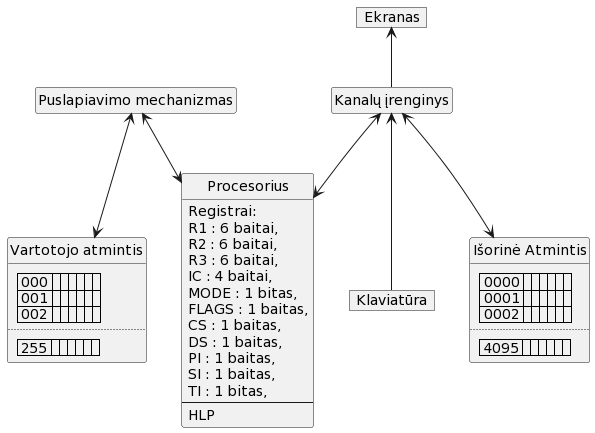
\includegraphics[scale=0.65]{img/reali_masina}
	\caption{Realios mašinos modelis}   % Antraštė įterpiama po paveikslėlio
	\label{img:reali_masina}
\end{figure}

Realios mašinos modelis yra pateikiamas \ref{img:reali_masina} paveiksliuke. Tolesnėse sekcijose bus plačiau aprašoma kiekviena šios mašinos dalis

\subsection{Procesorius}

Procesorius turi registrus:

\begin{itemize}
	\item IC - komandų skaitiklis - 4 baitai.
	\item R1, R2, R3 - bendrosios paskirties registrai iš 6 baitų (vienas žodis).
	\item MODE - 1 bito registras, kuris nurodo procesoriaus darbo rėžimą (0 - vartotojas, 1 - supervizorius)
	\item FLAGS - požymių  registras, susidedantis iš šių 2 bitų (nuo didžiausio iki mažiausio): 
	\begin{itemize}
		\item ZF - yra 1, jei aritmetinės operacijos rezultatas yra 0, o kitu atveju išvalomas.
		\item SF - nustatomas 1, jei aritmetinės oepracijos rezultatas yra teigiamas, o priešingu atveju - 0.
	\end{itemize}
	\item PI - 1 bito programinių pertraukimų registras.
	\item TI - 1 bito laikrodžio pertraukimas registras.
	\item SI - 1 bito ?sisteminių?/?supervizorinių? pertraukimų registras.
\end{itemize}

Be registrų procesorius dar turi šias dalis:
\begin{itemize}
	\item Aukšto lygio kalbos procesorius - HLP. Jis atsakingas už komandų apdorojimą.
	\item 
\end{itemize}

\subsection{Vartotojo atmintis}

Mašinos atminties dydis yra 16 blokų po 16 žodžių. Vieno žodžio ilgis yra 6 baitai.

\subsection{Taimerio mechanizmas}
Realioje mašinoje yra taimeris. Jis skirtas tam, kad viena užduotis nebūtų vykdoma daugiau nei 255 laiko momentų. Tam tikslui po kiekvienos operacijos yra sumažina TI reikšmė. Skirtingos operacijos užtrunka skirtingą laiko skaičių: išvedimo į kanalų įrenginį ar įvedimo į jį užima 5 laiko vienetus, o visos kitos - 1. Kai TI reikšmė pasiekia 1 yra sugeneruojamas taimerio pertraukimas ir valdymas perduodamas supervizoriui.

\subsection{Kanalų įrenginys}

Realioje mašinoje yra įvedimo įrenginys - klaviatūra ir išvedimo įrenginys - ekranas. Jie su procesorium komunikuoja per kanalų įrenginį. Įvydžius apsikeitimo komandą EXCHGE yra perkeliamas vienas blokas. Tam, kad būtų specifikuota, tai, kas bus perkeliama yra naudojami šie kanalų įrenginio registrai:

\begin{itemize}
	\item SB - 1 baito registras, kuriame saugas takelio, iš kurio bus kopijuojama numeris
	\item DB - 1 baito registras, kuriame saugas takelio, į kurį bus kopijuojama
	\item TYPE - 1 bito registras, kuriame nurodytas tipas objekto, kuris bus kopijuotas. 0 - procesoriaus atmintis, 1 - išorinė atmintis/srautas.
\end{itemize}

\subsection{Išorinė Atmintis}

Išorinė atmints yra realizuojama kietuoju disku. Jame yra 256 blokai po 16 žodžių.

Komunikacija su išorine atmintimi yra vykdoma per kanalų įrenginį.

\subsection{Klaviatūra}

Kiekvienas klaviatūros mygtuko paspaudimas generuoja sisteminius pertraukimus, t.y. nustato registro SI reikšmę į 1. 

Reali mašina įsimena paskutinį simbolį ir jį ligi simbolis yra perskaitomas. Kai tai nutinka vietoje simbolio yra įrašoma reikšmė 0. Jei tokiu metu yra bandoma skaityti, tai laikoma, kad tai nepavyko.

\subsection{Ekranas}

Į ekraną galima išvesti vieną žodį. Tam programa turi perkelti reikšmę į R1 ir iškviesti programinį pertraukimą

\section{Virtualios mašinos modelis}

\begin{figure}[H]
	\centering	
	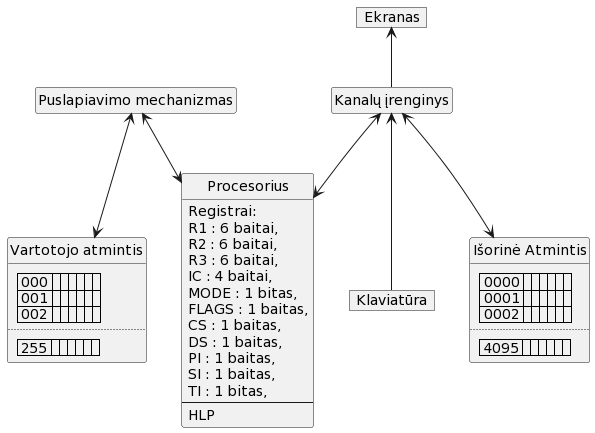
\includegraphics[scale=0.65]{img/reali_masina}
	\caption{Virtualios mašinos modelis}   % Antraštė įterpiama po paveikslėlio
	\label{img:virtuali_masina}
\end{figure}

Virtuali mašina - operacinės sistemos konstruktas, kurio pagalba kiekvienos programos veikimas yra izoliajamos nuo visų kitų. Šios mašinos modelis yra pateikiamas \ref{img:virtuali_masina} paveiksliuke.

\subsection{Registrai}

Virtuali mašina turi priėjimą tik prie šių realios mašinos registrų:

\begin{itemize}
	\item R1, R2, R3 (bendros paskirties registrai)
	\item FLAGS (požymių registras)
	\item IC (programos skaitiklis)
\end{itemize}

\subsection{Atmintis}

Virtuali mašina turi priėjimą prie 5 blokų. Virtuali mašina gauna blokų virtualius numerius. Dėl to kiekviena virtuali mašina mato, kad jos blokai yra pirmi penki - 0, 1, 2, 3, 4. Norint juos paversti į realios mašinos blokų numerius yra taikomas puslapiavimo mechanizmas. Jo metu procesorius pagal programos numerį ir jos puslapio numerį grąžina realų bloką.

\subsection{Komandos}

Visos komandos yra aprašomos vienu žodžiu - 6 baitais. Visose komandose simbolis * reiškia, kad šis baitas nėra naudojamas.

\subsubsection{Aritmetinės}
Po kiekvienos aritmetinės operacijos procesorius padina IC reikšmę.
\begin{itemize}
	\item ADDmxy - jei m = 0, tai operacija sudeda skaičius esančius registruose Rx, Ry ir rezultatą patalpina į R1.
	\item SUBmxy - jei m = 0, tai operacija atima iš skaičiaus esančio registre Rx, skaičių iš registro Ry ir rezultatą patalpina į R1. Jei m=1, tai operaciją atlieka su registru Rx ir konstanta y.
	\item MULmxy - jei m = 0, tai operacija sudaugina skaičius esančius registruose Rx, Ry ir rezultatą patalpina į R1. Jei m=1, tai operaciją atlieka su registru Rx ir konstanta y.
	\item DIVmxy - jei m = 0, tai operacija padalina skaičių esantį registre Rx, iš skaičiaus esančio registre Ry ir rezultatą patalpina į R1. Jei m=1, tai operaciją atlieka su registru Rx ir konstanta y.
	\item CMPmxy - jei m = 0, tai operacija palygina skaičius esančius registruose Rx ir Ry bei pagal Rx-Ry reikšmę nustato registro FLAGS reikšmę. Jei m=1, tai operaciją atlieka su registru Rx ir konstanta y.
\end{itemize}

\subsubsection{Duomenų judėjimo}
\begin{itemize}
	\item MVmxy - Perkelia duomenis. m reikšmė nurodo perkelimo režimą. x ir y specifikuoja vietas, kur juda duomenys. Po šios komandos yra padidinama IC reikšmė.
	\begin{enumerate}
		\item m=1. Šiuo atveju perkėlimas yra iš registro į registrą. x nurodo pirmo registro (šaltinio) numerį, y - tikslo.
		\item m = 2. Šiuo atveju perkėlimas yra iš registro R1 į atmintį. Atminties vieta yra gaunama pagal formulę $10 \cdot x + y$.
		\item m = 2. Šiuo atveju perkėlimas yra iš atminties į registrą R1. Atminties vieta yra gaunama pagal formulę $10 \cdot x + y$.
	\end{enumerate}(register <-> memory (arba reg <-> reg))
\end{itemize}

\subsubsection{Valdymo}
Norint tinkamai naudotis perėjimais, prieš juos reikia panaudoti CMP operaciją. 
\begin{itemize}
	\item JMPxyz - besąlyginis perėjimas. $x, y, z \in \{1, 2, \cdots 9 \}$. IC := 100*x + 10 * y + z.
	\item JExyz* - pereiti, jeigu lygu. $x, y, z \in \{1, 2, \cdots 9 \}$. Jei ZF=1, tai IC := 100*x + 10 * y + z, kitu atveju IC := IC + 1.
	\item JNExyz* - pereiti, jei nelygu. $x, y, z \in \{1, 2, \cdots 9 \}$. Jei ZF=0, tai IC := 100*x + 10 * y + z, kitu atveju IC := IC + 1.
	\item JLxyz* - pereiti, jeigu mažiau. $x, y, z \in \{1, 2, \cdots 9 \}$. Jei SF=1, tai IC := 100*x + 10 * y + z, kitu atveju IC := IC + 1.
	\item JLExyz* - pereiti, jeigu mažiau arba lygu. $x, y, z \in \{1, 2, \cdots 9 \}$. Jei ZF=1 arba SF=1, tai IC := 100*x + 10 * y + z, kitu atveju IC := IC + 1.
	\item JGxyz* - pereiti, jeigu daugiau. $x, y, z \in \{1, 2, \cdots 9 \}$. Jei SF=0, tai IC := 100*x + 10 * y + z, kitu atveju IC := IC + 1.
	\item JGExyz* - pereiti jeigu daugiau arba lygu. $x, y, z \in \{1, 2, \cdots 9 \}$. Jei ZF=1 arba SF=0, tai IC := 100*x + 10 * y + z, kitu atveju IC := IC + 1.
\end{itemize}

Po valdymo komandų registro FLAGS reikšmė nėra keičiama.

\subsubsection{Darbas su failais}
Darbo su failais metu yra naudojamos simbolių eilutės. Tai nulių besibaigianti baitų seka. Visos šios operacijos iškviečia programinius pertraukimus, o procesoriui reikalinga informacija apie komandos paskirtį yra gauname per komandos pavadinimą.
\begin{itemize}
	\item OPENF* - atidaro failą, kurio pavadinimas yra simbolių eilutė, kurios pradžios adresas yra R1 reikšmė. Operacijos pabaigoje į R2 yra įrašomas failo numeris. Jeigu failas yra nerandamas - nustato SI=1.
	\item CLOSEF - uždaro failą, kurio numeris yra įrašytas  R2. Jeigu norimas failas nėra rastas, ar jau buvo uždarytas yra nustatoma SI=1
	\item WRITEF - parašo simbolių eilutę, kurios adresas yra nurodytas R1 į failą, kurio numeris yra įrašytas į R2.
	\item READ* - perskaito simbolį iš failo ir jo reikšmę įrašo į R1. R2 - nuskaitomo failo numeris.
	\item DELETF - sunaikiną failą, kurio pavadimas yra simbolių eilutė, kurios pradžios adresas yra nurodomas R1 reikmšmėje.
\end{itemize}

Po kiekvienos iš šių komandų procesorius padidina registro IC reikšmę ir išvalo FLAGS registrą.

\subsubsection{Įvedimas ir išvedimas}
Įvedimo ir išvedimo komandos, kaip ir darbo su failais komandos, iškvieia programinį pertraukimą.
\begin{itemize}
	\item WRITEU - parašo simbolių eilutę, kurios pradžios adresas yra nurodytas registre R1 į ekraną.
	\item READU* - perskaito simbolį įvestą iš klaviatūros bei reikšmę patalpina į R1. Jeigu nuskaityti nepavyko, tai gauname reikšmė R1=0.
\end{itemize}

\subsubsection{Programos pabaigos}
\begin{itemize}
	\item HALT - baigia programos darbą.
\end{itemize}

\subsubsection{Neaptartos situacijos}

Jeigu programos vykdymo metu yra sutinkama komanda, kurios procesorius nesugeba apdoroti, tai jokia programa nėra vykdoma ir padidinama IC reikšmė.

Jei programos vykdymo metu IC reikšmė viršija 79 (programos žodžių skaičius), tai programa yra nutraukiama.

\subsection{Programos struktūra}

Programos pradžią žymi žodis \$START, o pabaigą - \$FINSH. Tarp šių žodžių yra rašomos programos komandos. Jos užima vieta kode nuo programos pradžios. 

Nuo žymės .DTSEG yra duomenų segmento vieta. Nuo šios vietos tolesni žodžiai programos darbo pradžioje yra užpildomi nuliais, nebent po duomenų segmento žymės neseka programos pabaigos žymė. Tokiu atveju visi tarpiniai žodžiai yra įdedami į programą.

Žymė .START žymi vykdomojo kodo pradžią. Kai programa yra perkeliama į vartotojo atmintį, yra nustatoma tokia IC reikšmė, kad  atminties ląstelėje su adresu IC – 1 būtų ši žymė. Jei programoje nėra, ar yra daugiau nei 1 .START žymė, tai programos įkėlimas į atmintį baigiasi klaida.

\subsection{Virtuali mašina operacinės sistemos kontekste}

Operacinė sistema paleidžia virtualią mašiną kiekvienai programai. Jei operacinė sistema yra multiprograminė, tai joje vienu metu veikia tik viena programa, bet vykdomoji programa nuolatos keičiasi.

Virtualias mašinas kuria operacinė sistemą. Jos yra sukuriamos, kai vartotojas įveda programą LOAD prg, kur prg yra programos pavadinimas kietąjame diske.

\printbibliography[heading=bibintoc] % Literatūros šaltiniai aprašomi
\appendix  % Priedai

\end{document}
